\begin{enumerate}
    \item Not-Aus drücken!
    \item Ladedeckel öffnen
    \item Ladegerät anschließen
    \item Ladevorgang starten siehe \ref{sec: bilderanleitung_laden}
    \item Ladegerät abschließen \& Kabel in Ladebox verstauen
    \item Ladedeckel schließen
\end{enumerate}

\newpage
\section{Bilderanleitung Ladevorgang \label{sec: bilderanleitung_laden}}
Die Bedienung des Ladegerätes ist im Folgenden dargestellt. \\

In \autoref{fig:Ladegeraet_Hauptanzeige} lässt sich die Hauptanzeige des Ladegeräts erkennen, welche 
sofort erscheint, wenn die Akkus angeschlossen sind. 


\begin{figure}[H]
    \centering
    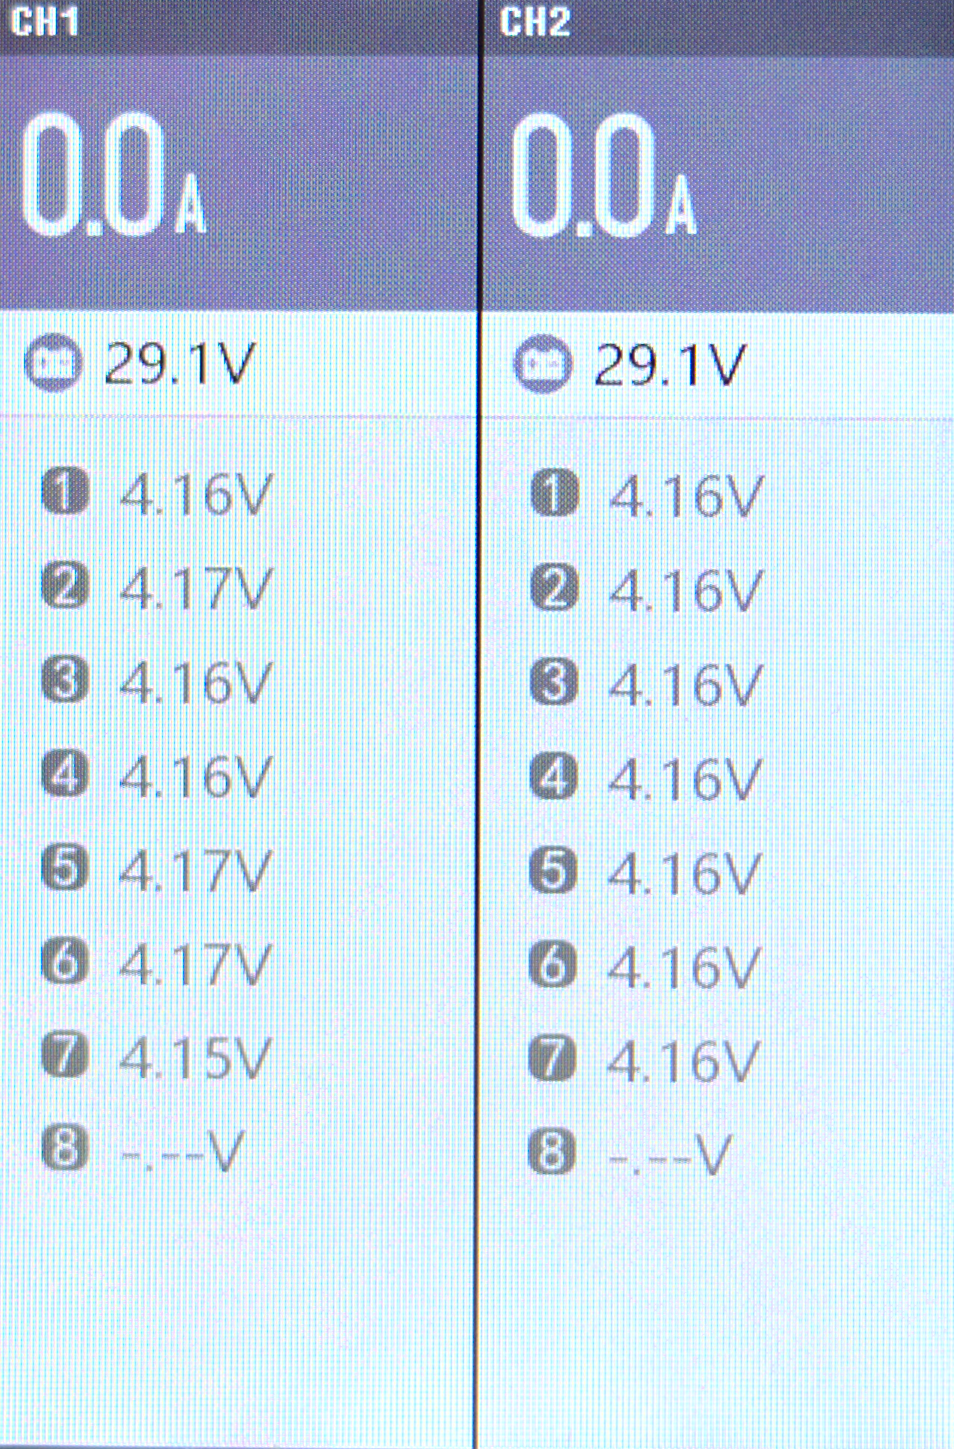
\includegraphics[width=.35\textwidth]{Fotos/Ladegereat/DSC_8742_Ladegereat_Hauptanzeige.png}
    \caption{Ladegerät Hauptanzeige \label{fig:Ladegeraet_Hauptanzeige}}
\end{figure}

\begin{figure}[H]
    \centering
    \includegraphics[width=.35\textwidth]{Fotos/Ladegereat/DSC_8744_Lademenue.png}
    \caption{Ladegerät Menüanzeige}
\end{figure}

\begin{figure}[H]
    \centering
    \includegraphics[width=.35\textwidth]{Fotos/Ladegereat/DSC_8745_Lademenue_2.png}
    \caption{Ladegerät Menüanzeige 2}
\end{figure}

\begin{figure}[H]
    \centering
    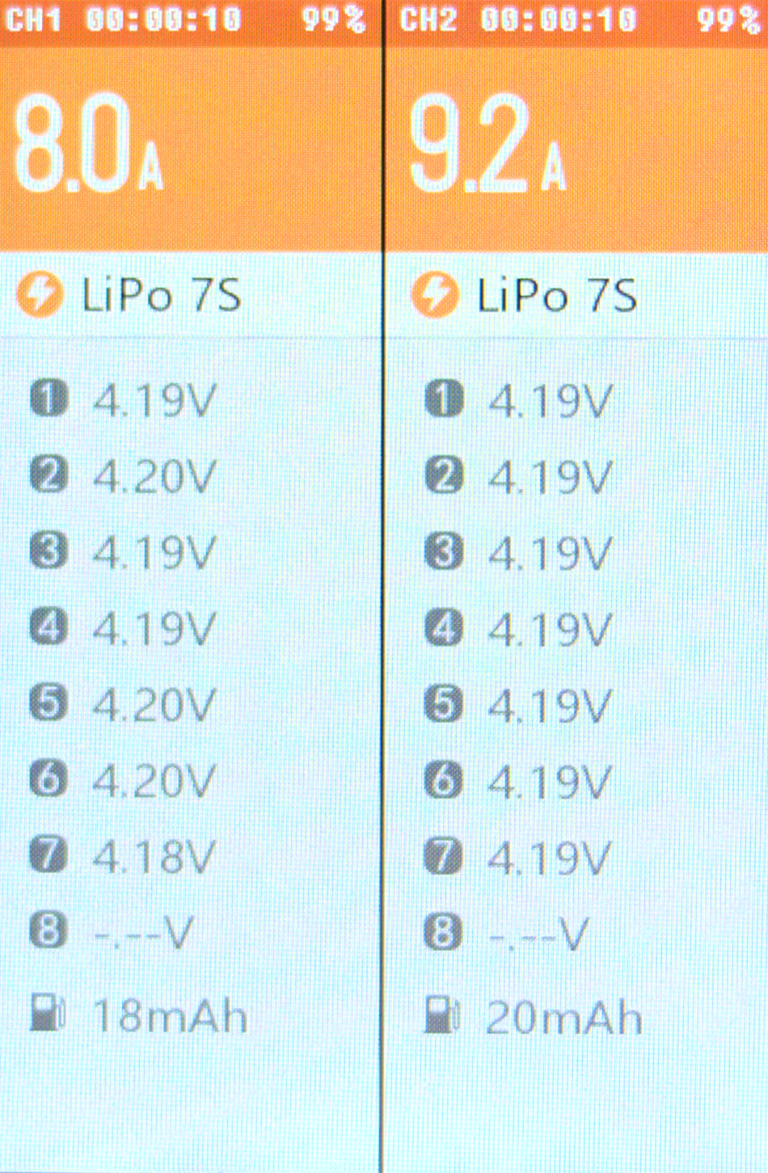
\includegraphics[width=.35\textwidth]{Fotos/Ladegereat/DSC_8747_Laden.png}
    \caption{Ladegerät Ladezustand}
\end{figure}

 \todo{das zu einer section machen?}